\section{QSAES18}

\begin{frame}{QSAES18}

\begin{figure}[h!]
    \centering
    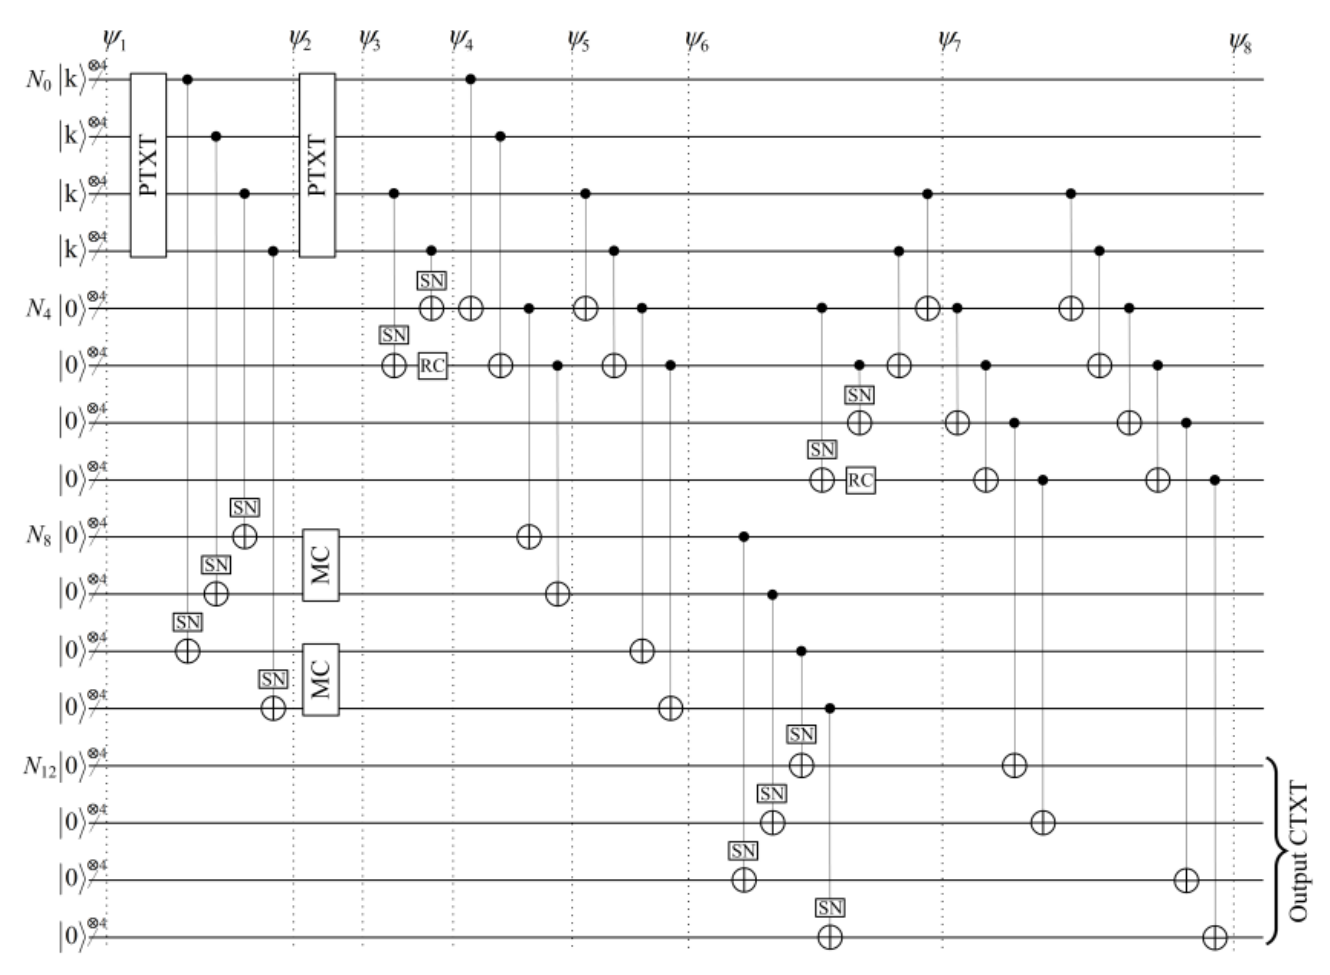
\includegraphics[width=0.8\linewidth]{saes18/qsaes18.png}
    \caption{QSAES18\footfullcite{Almazrooie}}
    \label{fig:qaes18}
\end{figure}

\end{frame}

\begin{frame}{Sub Nibbles}
    Fermat inversion algorithm (square and multiply method) to find multiplicative inverse in $GF(2^4)$
    \pause
    \begin{equation*}
        x^{-1} = x^{2^4 - 2} = x^{16-2} = x^{14} = x^{2} \times (x^{2})^{2} \times ((x^{2})^{2})^{2}
    \end{equation*}
    \pause
    \begin{figure}[h!]
        \centering
        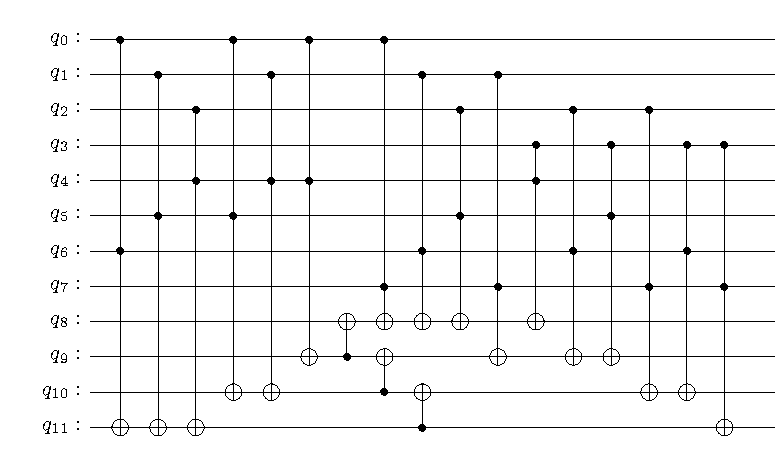
\includegraphics[width=0.5\linewidth]{saes18/multiplier.pdf}
        \caption{Multiplier\footfullcite{Cheung} }
        \label{fig:mul}
    \end{figure}
    Input: $q_0 - q_3$ and $q_4 - q_7$. Output: $q_8 - q_{11}$.
\end{frame}
\begin{frame}{Sub Nibbles Contd.}
Squarer circuit obtained using CNOT synthesis algorithm.

\begin{figure}[h!]
    \centering
    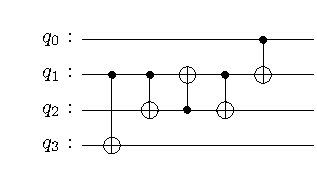
\includegraphics[width=0.4\linewidth]{saes18/squarer.pdf}
    \caption{Squarer}
    \label{fig:sq}
\end{figure}

Affine transformation circuit.
\begin{figure}[h!]
    \centering
    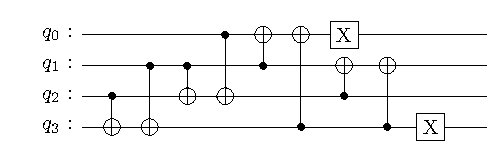
\includegraphics[width=0.7\linewidth]{saes18/affine.pdf}
    \caption{Affine transformation}
    \label{fig:aff}
\end{figure}
\end{frame}

\begin{frame}{Sub Nibbles Complete Circuit}
    \begin{figure}[h!]
    \centering
    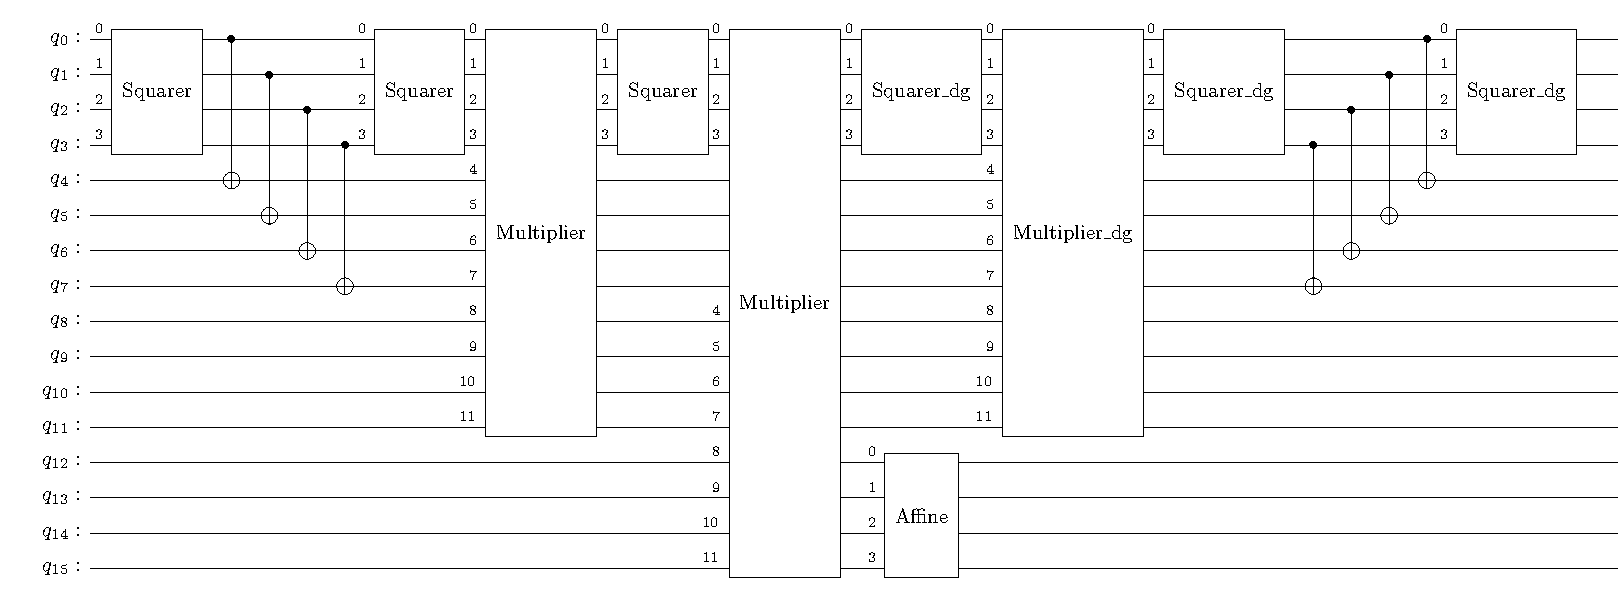
\includegraphics[width=1\linewidth]{saes18/sbox.pdf}
    \caption{Sbox}
    \label{fig:sb}
\end{figure}
\end{frame}
\begin{frame}{Mix Column}
Obtained using CNOT synthesis algorithm.
\begin{figure}[h!]
    \centering
    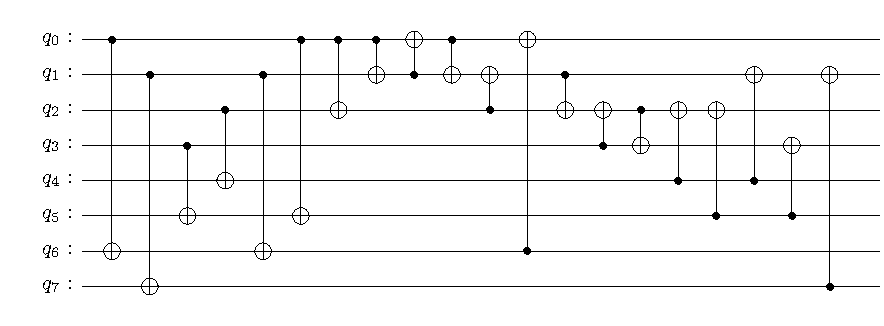
\includegraphics[width=1\linewidth]{saes18/mc.pdf}
    \caption{Mix column}
    \label{fig:mc}
\end{figure}
The circuit takes 1 byte (1 column of the state matrix) and outputs the corresponding matrix multiplication in $GF(2^4)$.
\end{frame}
\begin{frame}{Grover's Attack}
    Boolean function for Grover's oracle:
    \begin{equation*}
     f(k) = 
     \begin{cases} 
          1 & SAES(k, p) = c\\
          0 & else 
      \end{cases}
    \end{equation*}
    \pause
   
    \begin{figure}[h!]
    \begin{center}
 \resizebox{10cm}{!}{
\begin{quantikz}
\lstick{$\ket{0}^{\otimes 16}$\\key} &[2mm]\gate{H^{\otimes 16}}\slice{$\ket{\psi_1}$} & \gate[wires=2][2cm]{P~SAES} & \qw & \qw \slice{$\ket{\psi_2}$}& \qw & \gate[wires=2][2cm]{P~SAES^\dagger}\slice{$\ket{\psi_3}$} & \gate{INV}\slice{$\ket{\psi_4}$} & \qw \\
\lstick{$\ket{0}^{\otimes 63}$\\work space} &[2mm] \qw & & \gate{C} & \ctrl{1} & \gate{C} & & \qw & \qw \\
\lstick{$\ket{0}$\\oracle} &[2mm] \gate{X} & \gate{H} & \qw & \targ{} & \qw & \qw & \qw & \qw 
\end{quantikz}}
\end{center}
    \caption{Grover's Attack on SAES}
    \label{fig:grov18}
\end{figure}
\pause
Number of iterations:
\begin{equation}
    t = \frac{\pi}{4}\sqrt{\frac{2^k}{s}}
\end{equation}
$s = 2, k = 16$
\begin{equation*}
    t = \frac{\pi}{4}\sqrt{\frac{2^{16}}{2}} = 142
\end{equation*}
\end{frame}
\begin{frame}{Grover's Attack (r = 2)}
They propose a modified version of Grover's Attack to find the unique key which is shown below.
    \begin{figure}[h!]
    
    \resizebox{10cm}{!}{
    \begin{quantikz}
    \lstick{$\ket{0}^{\otimes 16}$\\key} &[2mm]\gate{H^{\otimes 16}} & \gate[wires=2][2cm]{P_1~SAES} & \qw & \qw & \qw & \gate[wires=2][2cm]{P_1~SAES^\dagger} & \gate[wires=2][2cm]{P_2~SAES} & \qw & \qw &\qw & \gate[wires=2][2cm]{P_2~SAES^\dagger}& \gate[wires=2][2cm]{P_1~SAES} & \qw & \qw & \qw & \gate[wires=2][2cm]{P_1~SAES^\dagger} & \gate{INV} & \qw \\
    \lstick{$\ket{0}^{\otimes 63}$\\work space} &[2mm] \qw & & \gate{C_1} & \ctrl{1} & \gate{C_1} & & \qw & \gate{C_2} & \ctrl{2} & \gate{C_2} &\qw &\qw & \gate{C_1} & \ctrl{1} & \gate{C_1} & \qw & \qw & \qw  \\
    \lstick{$\ket{0}$\\oracle} &[2mm]  \qw & \qw & \qw &\targ{}&  \qw & \qw & \qw  & \qw& \control{} & \qw & \qw & \qw & \qw &\targ{}  &  \qw &  \qw &  \qw & \qw   \\
    \lstick{$\ket{0}$\\oracle} &[2mm] \gate{X} & \gate{H} & \qw & \qw & \qw & \qw  & \qw & \qw &\targ{} & \qw & \qw & \qw & \qw & \qw & \qw & \qw &\qw &\qw
    \end{quantikz}
    }
    
    \caption{Grover's Attack to find unique key with r = 2}
    \label{fig:grov18u}
\end{figure}
\pause
The corresponding boolean function is described as follows:
\begin{equation*}
 f(k) = 
 \begin{cases} 
      1 & (SAES(k, p_1) = c_1) \wedge (SAES(k, p_2) = c_2) \\
      0 & else 
  \end{cases}
\end{equation*}
\end{frame}